\documentclass[border=3pt,tikz]{standalone}
\usepackage{amsmath}
\usetikzlibrary{calc}
\usetikzlibrary{arrows.meta} % for arrow size
\begin{document}
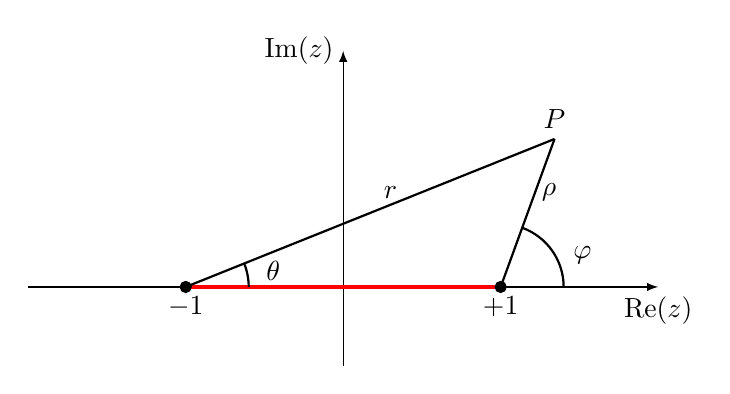
\begin{tikzpicture}[scale=2]
    \usetikzlibrary {arrows.meta}
    \usetikzlibrary {calc}
    
    \coordinate (z1) at (1, 0);
    \coordinate (z2) at (-1, 0);
    \coordinate (P) at ({1+ cos(70)}, {sin(70)});
    \draw [-latex] (-2, 0) -- (2, 0) node[below] {Re$(z)$};
    \draw [-latex] (0, -0.5) -- (0, 1.5) node[left] {Im$(z)$};
    
    \draw [red, very thick] (z1) -- (z2) ; 
    \draw [thick] (z1) -- (P) node[above] {$P$};
    \draw [thick] (P) -- (z2);
    
    \draw[thick, ] (-0.6, 0) arc (0:21.86:0.4);
    \node [right] at (-0.55, 0.1) {$\theta$};
    
    \draw[thick, ] (1.4, 0) arc (0:70:0.4);
    \node [right] at (1.4, 0.2) {$\varphi$};
    
    
    \filldraw [] (z1) circle (1pt) node [below] {$+1$} ;
    \filldraw [] (z2) circle (1pt) node [below] {$-1$} ;
    
    \node [above] at (0.3, 0.5) {$r$};
    
    \node [right] at (1.2, 0.6) {$\rho$};
    
    \end{tikzpicture}
\end{document}